\documentclass{standalone}
\usepackage{tikz}
\usetikzlibrary{patterns, positioning}


\begin{document}
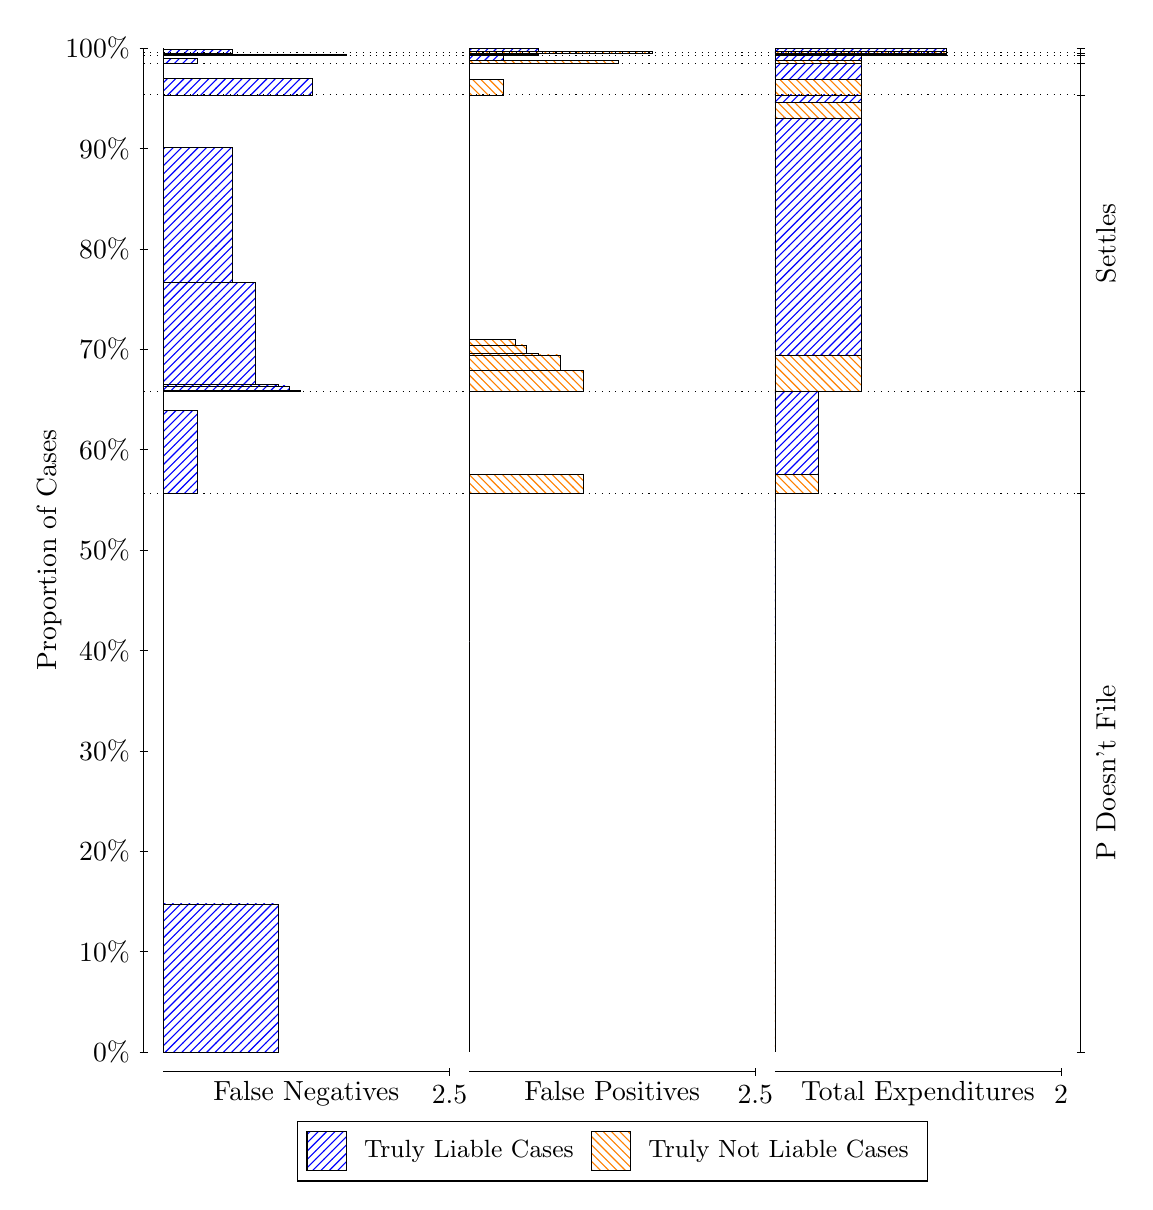
\begin{tikzpicture}
\draw[black, very thin] (1.5,1.75) -- (1.5,14.5);
\node[rotate=90, text=black, anchor=center] at (0.3, 8.125) {Proportion of Cases};
\draw[black, very thin] (1.45,1.75) -- (1.55,1.75);
\node[text=black, anchor=east] at (1.45, 1.75) {0\%};
\draw[black, very thin] (1.45,3.025) -- (1.55,3.025);
\node[text=black, anchor=east] at (1.45, 3.025) {10\%};
\draw[black, very thin] (1.45,4.3) -- (1.55,4.3);
\node[text=black, anchor=east] at (1.45, 4.3) {20\%};
\draw[black, very thin] (1.45,5.575) -- (1.55,5.575);
\node[text=black, anchor=east] at (1.45, 5.575) {30\%};
\draw[black, very thin] (1.45,6.85) -- (1.55,6.85);
\node[text=black, anchor=east] at (1.45, 6.85) {40\%};
\draw[black, very thin] (1.45,8.125) -- (1.55,8.125);
\node[text=black, anchor=east] at (1.45, 8.125) {50\%};
\draw[black, very thin] (1.45,9.4) -- (1.55,9.4);
\node[text=black, anchor=east] at (1.45, 9.4) {60\%};
\draw[black, very thin] (1.45,10.675) -- (1.55,10.675);
\node[text=black, anchor=east] at (1.45, 10.675) {70\%};
\draw[black, very thin] (1.45,11.95) -- (1.55,11.95);
\node[text=black, anchor=east] at (1.45, 11.95) {80\%};
\draw[black, very thin] (1.45,13.225) -- (1.55,13.225);
\node[text=black, anchor=east] at (1.45, 13.225) {90\%};
\draw[black, very thin] (1.45,14.5) -- (1.55,14.5);
\node[text=black, anchor=east] at (1.45, 14.5) {100\%};

\draw[black, very thin] (13.4,1.75) -- (13.4,14.5);
\draw[black, very thin] (13.35,1.75) -- (13.45,1.75);
\node[anchor=west] at (13.35, 1.75) {};
\draw[black, very thin] (13.35,8.8443) -- (13.45,8.8443);
\node[anchor=west] at (13.35, 8.8443) {};
\draw[black, very thin] (13.35,10.135) -- (13.45,10.135);
\node[anchor=west] at (13.35, 10.135) {};
\draw[black, very thin] (13.35,13.905) -- (13.45,13.905);
\node[anchor=west] at (13.35, 13.905) {};
\draw[black, very thin] (13.35,14.309) -- (13.45,14.309);
\node[anchor=west] at (13.35, 14.309) {};
\draw[black, very thin] (13.35,14.406) -- (13.45,14.406);
\node[anchor=west] at (13.35, 14.406) {};
\draw[black, very thin] (13.35,14.439) -- (13.45,14.439);
\node[anchor=west] at (13.35, 14.439) {};
\draw[black, very thin] (13.35,14.5) -- (13.45,14.5);
\node[anchor=west] at (13.35, 14.5) {};

\draw[black, very thin, pattern color=blue, pattern=north east lines] (1.75,1.75) rectangle (3.2033,3.6314);
\draw[black, very thin, pattern color=orange, pattern=north west lines] (1.75,3.6314) rectangle (1.75,8.8443);
\draw[black, very thin, pattern color=blue, pattern=north east lines] (1.75,8.8443) rectangle (2.186,9.897);
\draw[black, very thin, pattern color=orange, pattern=north west lines] (1.75,9.897) rectangle (1.75,10.135);
\draw[black, very thin, pattern color=blue, pattern=north east lines] (1.75,10.135) rectangle (3.494,10.149);
\draw[black, very thin, pattern color=blue, pattern=north east lines] (1.75,10.149) rectangle (3.3487,10.21);
\draw[black, very thin, pattern color=blue, pattern=north east lines] (1.75,10.21) rectangle (3.2033,10.233);
\draw[black, very thin, pattern color=blue, pattern=north east lines] (1.75,10.233) rectangle (2.9127,11.523);
\draw[black, very thin, pattern color=blue, pattern=north east lines] (1.75,11.523) rectangle (2.622,13.243);
\draw[black, very thin, pattern color=orange, pattern=north west lines] (1.75,13.243) rectangle (1.75,13.905);
\draw[black, very thin, pattern color=blue, pattern=north east lines] (1.75,13.905) rectangle (3.6393,14.113);
\draw[black, very thin, pattern color=orange, pattern=north west lines] (1.75,14.113) rectangle (1.75,14.309);
\draw[black, very thin, pattern color=blue, pattern=north east lines] (1.75,14.309) rectangle (2.186,14.372);
\draw[black, very thin, pattern color=orange, pattern=north west lines] (1.75,14.372) rectangle (1.75,14.406);
\draw[black, very thin, pattern color=blue, pattern=north east lines] (1.75,14.406) rectangle (4.0753,14.421);
\draw[black, very thin, pattern color=orange, pattern=north west lines] (1.75,14.421) rectangle (1.75,14.439);
\draw[black, very thin, pattern color=blue, pattern=north east lines] (1.75,14.439) rectangle (2.622,14.486);
\draw[black, very thin, pattern color=orange, pattern=north west lines] (1.75,14.486) rectangle (1.75,14.5);
\draw[black, very thin, pattern color=orange, pattern=north west lines] (5.6333,1.75) rectangle (5.6333,6.9629);
\draw[black, very thin, pattern color=blue, pattern=north east lines] (5.6333,6.9629) rectangle (5.6333,8.8443);
\draw[black, very thin, pattern color=orange, pattern=north west lines] (5.6333,8.8443) rectangle (7.0867,9.0822);
\draw[black, very thin, pattern color=blue, pattern=north east lines] (5.6333,9.0822) rectangle (5.6333,10.135);
\draw[black, very thin, pattern color=orange, pattern=north west lines] (5.6333,10.135) rectangle (7.0867,10.402);
\draw[black, very thin, pattern color=orange, pattern=north west lines] (5.6333,10.402) rectangle (6.796,10.603);
\draw[black, very thin, pattern color=orange, pattern=north west lines] (5.6333,10.603) rectangle (6.5053,10.62);
\draw[black, very thin, pattern color=orange, pattern=north west lines] (5.6333,10.62) rectangle (6.36,10.731);
\draw[black, very thin, pattern color=orange, pattern=north west lines] (5.6333,10.731) rectangle (6.2147,10.797);
\draw[black, very thin, pattern color=blue, pattern=north east lines] (5.6333,10.797) rectangle (5.6333,13.905);
\draw[black, very thin, pattern color=orange, pattern=north west lines] (5.6333,13.905) rectangle (6.0693,14.101);
\draw[black, very thin, pattern color=blue, pattern=north east lines] (5.6333,14.101) rectangle (5.6333,14.309);
\draw[black, very thin, pattern color=orange, pattern=north west lines] (5.6333,14.309) rectangle (7.5227,14.343);
\draw[black, very thin, pattern color=blue, pattern=north east lines] (5.6333,14.343) rectangle (6.0693,14.406);
\draw[black, very thin, pattern color=orange, pattern=north west lines] (5.6333,14.406) rectangle (6.5053,14.424);
\draw[black, very thin, pattern color=blue, pattern=north east lines] (5.6333,14.424) rectangle (5.6333,14.439);
\draw[black, very thin, pattern color=orange, pattern=north west lines] (5.6333,14.439) rectangle (7.9587,14.453);
\draw[black, very thin, pattern color=blue, pattern=north east lines] (5.6333,14.453) rectangle (6.5053,14.5);
\draw[black, very thin, pattern color=orange, pattern=north west lines] (9.5167,1.75) rectangle (9.5167,6.9629);
\draw[black, very thin, pattern color=blue, pattern=north east lines] (9.5167,6.9629) rectangle (9.5167,8.8443);
\draw[black, very thin, pattern color=orange, pattern=north west lines] (9.5167,8.8443) rectangle (10.062,9.0822);
\draw[black, very thin, pattern color=blue, pattern=north east lines] (9.5167,9.0822) rectangle (10.062,10.135);
\draw[black, very thin, pattern color=orange, pattern=north west lines] (9.5167,10.135) rectangle (10.607,10.603);
\draw[black, very thin, pattern color=blue, pattern=north east lines] (9.5167,10.603) rectangle (10.607,13.613);
\draw[black, very thin, pattern color=orange, pattern=north west lines] (9.5167,13.613) rectangle (10.607,13.807);
\draw[black, very thin, pattern color=blue, pattern=north east lines] (9.5167,13.807) rectangle (10.607,13.905);
\draw[black, very thin, pattern color=orange, pattern=north west lines] (9.5167,13.905) rectangle (10.607,14.101);
\draw[black, very thin, pattern color=blue, pattern=north east lines] (9.5167,14.101) rectangle (10.607,14.309);
\draw[black, very thin, pattern color=orange, pattern=north west lines] (9.5167,14.309) rectangle (10.607,14.343);
\draw[black, very thin, pattern color=blue, pattern=north east lines] (9.5167,14.343) rectangle (10.607,14.406);
\draw[black, very thin, pattern color=orange, pattern=north west lines] (9.5167,14.406) rectangle (11.697,14.424);
\draw[black, very thin, pattern color=blue, pattern=north east lines] (9.5167,14.424) rectangle (11.697,14.439);
\draw[black, very thin, pattern color=orange, pattern=north west lines] (9.5167,14.439) rectangle (11.697,14.453);
\draw[black, very thin, pattern color=blue, pattern=north east lines] (9.5167,14.453) rectangle (11.697,14.5);
\draw[black, dotted] (1.5,8.8443) -- (13.4,8.8443);
\draw[black, dotted] (1.5,10.135) -- (13.4,10.135);
\draw[black, dotted] (1.5,13.905) -- (13.4,13.905);
\draw[black, dotted] (1.5,14.309) -- (13.4,14.309);
\draw[black, dotted] (1.5,14.406) -- (13.4,14.406);
\draw[black, dotted] (1.5,14.439) -- (13.4,14.439);
\draw[black, very thin] (1.75,1.5) -- (5.3833,1.5);
\node[text=black, anchor=north] at (3.5667, 1.5) {False Negatives};
\draw[black, very thin] (5.3833,1.45) -- (5.3833,1.55);
\node[text=black, anchor=north] at (5.3833, 1.45) {2.5};

\draw[black, very thin] (5.6333,1.5) -- (9.2667,1.5);
\node[text=black, anchor=north] at (7.45, 1.5) {False Positives};
\draw[black, very thin] (9.2667,1.45) -- (9.2667,1.55);
\node[text=black, anchor=north] at (9.2667, 1.45) {2.5};

\draw[black, very thin] (9.5167,1.5) -- (13.15,1.5);
\node[text=black, anchor=north] at (11.333, 1.5) {Total Expenditures};
\draw[black, very thin] (13.15,1.45) -- (13.15,1.55);
\node[text=black, anchor=north] at (13.15, 1.45) {2};

\node[text=black, centered, rotate=90] at (13.72, 5.2972) {P Doesn't File};

\node[text=black, centered, rotate=90] at (13.72, 12.02) {Settles};





\draw (7.449999999999999,1.5) node[draw=none] (baseCoordinate) {};
\begin{scope}[align=center]
        \matrix[scale=0.5, draw=black, below=0.5cm of baseCoordinate, nodes={draw}, column sep=0.1cm]{
            \node[rectangle, draw, minimum width=0.5cm, minimum height=0.5cm, pattern color=blue, pattern=north east lines] {}; &
            \node[draw=none, font=\small, text=black] (B) {Truly Liable Cases}; &
            \node[rectangle, draw, minimum width=0.5cm, minimum height=0.5cm, pattern color=orange, pattern=north west lines] {}; &
            \node[draw=none, font=\small, text=black] (B) {Truly Not Liable Cases}; \\
            };
\end{scope}

\end{tikzpicture}
\end{document}